\documentclass[spanish]{beamer}
\usepackage[utf8]{inputenc}
\usepackage[spanish]{babel}

\usepackage{default}
\usetheme{Boadilla}

\usepackage{multicol}
\usepackage{textcomp}	

\title[MDIAE]{Software Libre en el ámbito espacial}
\author{Arias Emmanuel}
\institute[EILAR 2018]{Encuentro informático 2018}
\date{La Rioja, 2018}

\begin{document}
	
\begin{frame}
	\titlepage
\end{frame}

	
\begin{frame}%[allowframebreaks]
	\frametitle{Agenda}
	\begin{multicols}{2}
		\tableofcontents
	\end{multicols}
\end{frame}

\AtBeginSection[]
{
	\begin{frame}%[allowframebreaks]
		\frametitle{Agenda}
		\begin{multicols}{2}
			\tableofcontents[currentsection]
		\end{multicols}
	\end{frame}
}
\AtBeginSubsection[]
{
	\begin{frame}%[allowframebreaks]
		\frametitle{Agenda}
		\begin{multicols}{2}
			\tableofcontents[currentsubsection]	
		\end{multicols}
	\end{frame}
}
\section{Me presento}
\begin{frame}
	\frametitle{Hola... :-)}
	\begin{itemize}
		\item Licenciado (2014) e Ingeniero (2015) recibido de UNLAR. 
		\item Becas de Verano del Instituto Balseiro en 2015. (Teleoperación háptica de	robots en ambientes	simulados)
		\item Maestría en Desarrollo Informático de Aplicación Espacial (2015): Tesis: Diseño de una arquitectura tolerante a fallas basadas en componentes COTS para vehículo satelitales de nueva generación. 
		\item Veng S.A. (2017) - principal proveedora de CONAE (Comisión Nacional de Actividades Espaciales.)
		\item Octubre 2018 se Lanza del SAOCOM 1A.
	\end{itemize}
\end{frame}

\begin{frame}
	\frametitle{Contribuciones en el software libre}
	\begin{figure}
		\centering
		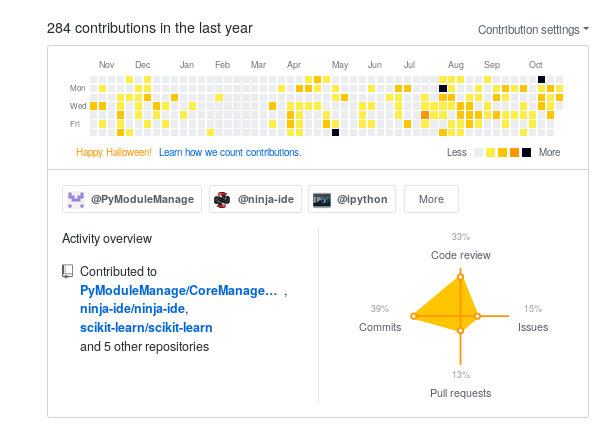
\includegraphics[width=0.7\linewidth]{contributions}
		\label{fig:contributions}
	\end{figure}
\end{frame}

\begin{frame}
	\frametitle{Un poco de Machine Learning}
	\begin{figure}
		\centering
		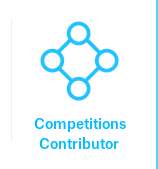
\includegraphics[width=0.3\linewidth]{kaggle}
	\end{figure}
\end{frame}

\begin{frame}
	\frametitle{Y un poco en Debian}
	\begin{figure}
		\centering
		
\includegraphics[width=0.4\linewidth]{Debian}
	\end{figure}
\end{frame}
\section{Software libre}
\begin{frame}
	\begin{figure}
		\centering
		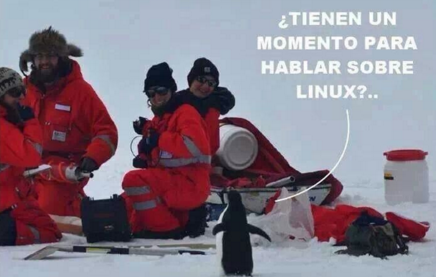
\includegraphics[width=0.9\linewidth]{tux-evang}
	\end{figure}
\end{frame}
\begin{frame}
	\frametitle{El software libre debe cumplir con las siguientes leyes:}
	\begin{multicols}{2}
		\begin{itemize}
			\item Libertad 0: Es la libertad de ejecutar un programa como se desee, y para cualquier propósito
			\item Libertad 1: Es la libertad de estudiar como funciona un programa, y realizar modificaciones. Para ello es necesario poder acceder al código fuente.
			\item Libertad 2: Es la libertad de redistribuir copias, con esto, se puede ayudar a las demas personas.
			\item Libertad 3: Es la libertad de distribuir copias de versiones modificadas del software original. Con esto se le brinda a la comunidad la oportunidad de beneficiarse por los cambios realizados en el software.
		\end{itemize}
	
	\begin{figure}
		\centering
		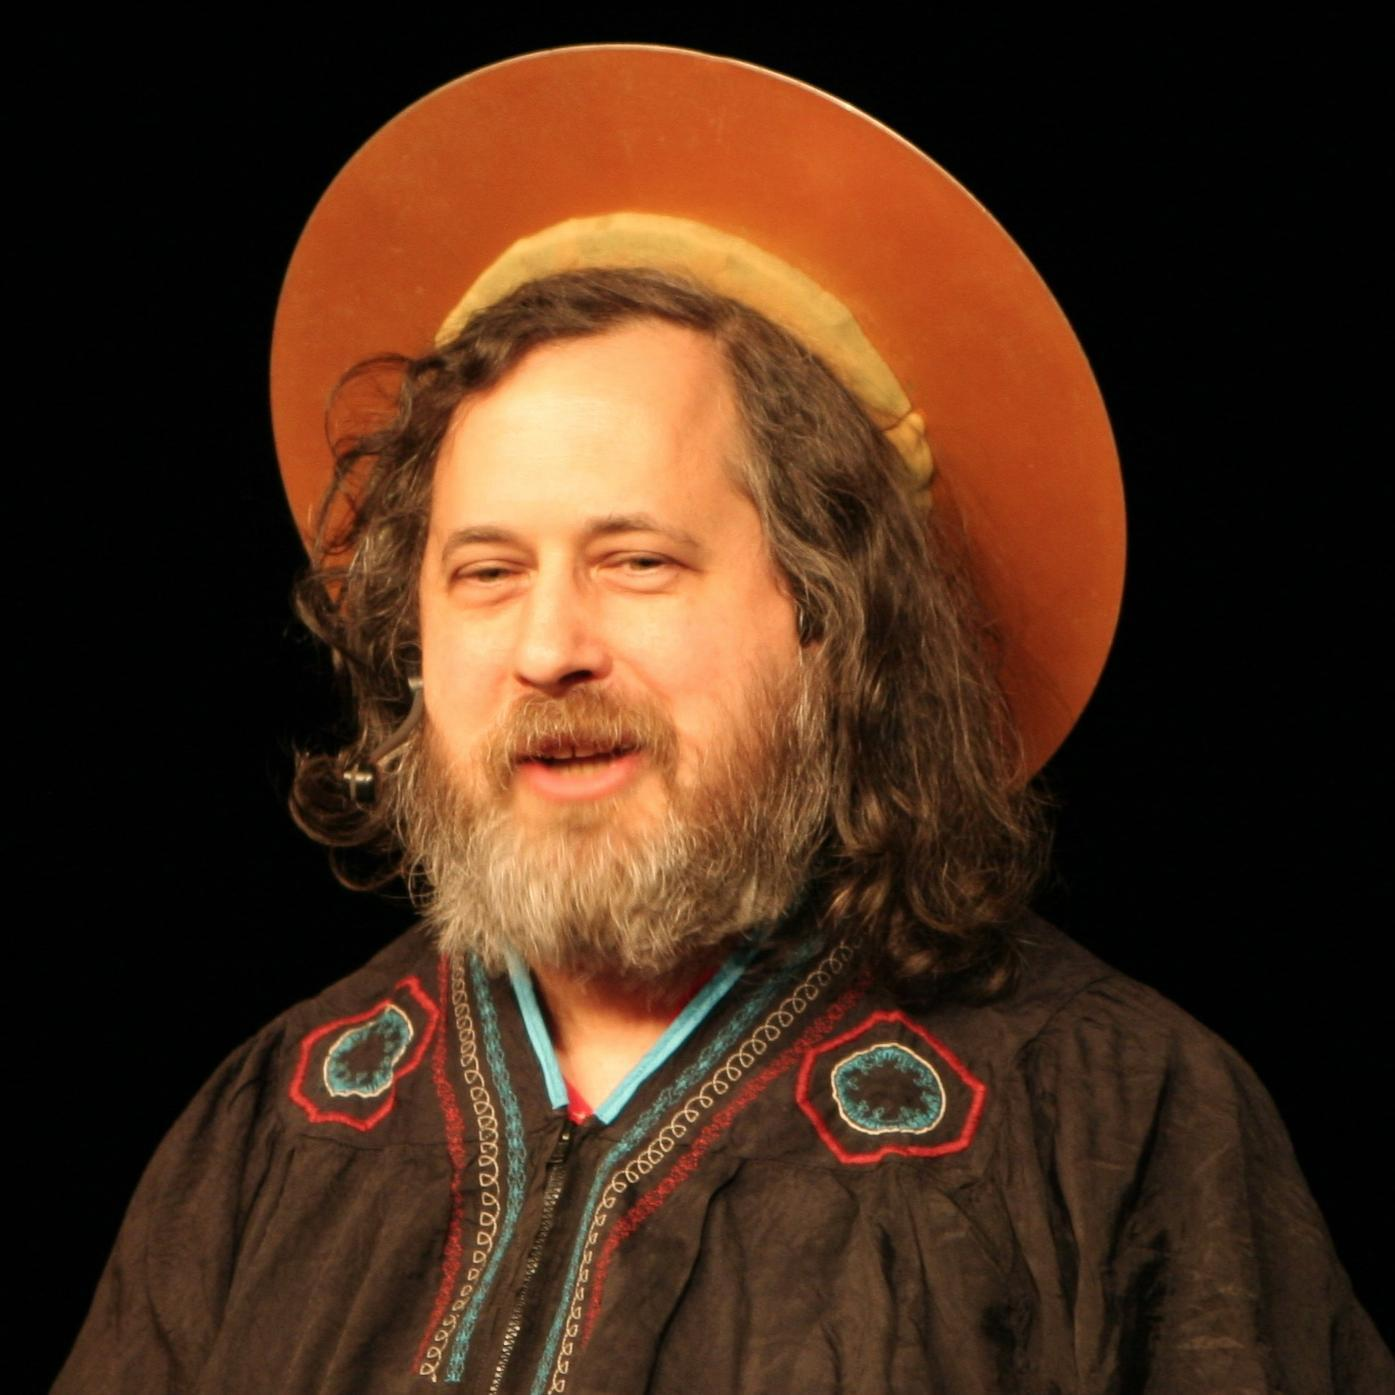
\includegraphics[width=0.7\linewidth]{stallman}
	\end{figure}
	\end{multicols}
	\end{frame}

\section{Open Source}
\begin{frame}
	\begin{multicols}{2}
		\begin{itemize}
			\item El Software Libre nació en 1983
			\item En 1998 nace el Open Source
			\item Nace con la intención de no asustar a las empresas con el software libre
			\item Hay que tener en cuenta que el Software libre es un movimiento, y el open source es una metodología
		\end{itemize}
	\begin{figure}
		\centering
		
\includegraphics[width=0.7\linewidth]{Opensource}
	\end{figure}
	\end{multicols}
\end{frame}
\section{Algunos softwares utilizados}
\subsection{Papyrus}
\begin{frame}
	\frametitle{Papyrus}
	\begin{figure}
		\centering
		
\includegraphics[width=0.3\linewidth]{../Resumen/papyrus}
	\end{figure}
	\begin{figure}
		\centering
		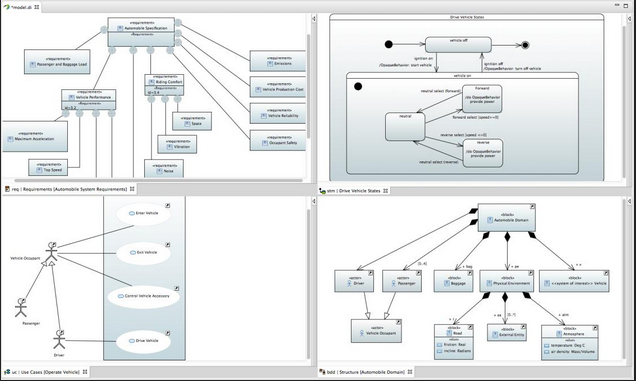
\includegraphics[width=0.6\linewidth]{../Resumen/papyrus2}
	\end{figure}
\end{frame}

\subsection{GPredict}
\begin{frame}
	\frametitle{GPredict}
\begin{figure}
	\centering
	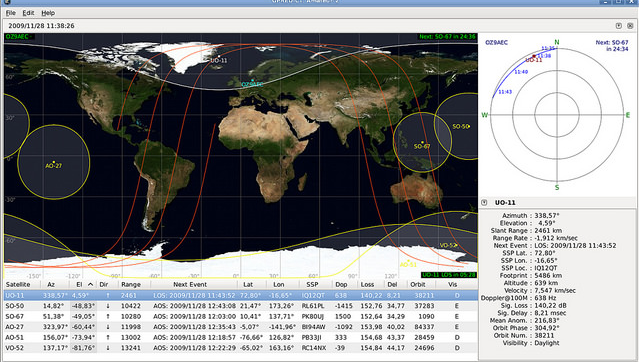
\includegraphics[width=1\linewidth]{../Resumen/gpredict}
\end{figure}
\end{frame}

\subsection{FreeRTOS}
\begin{frame}
	\frametitle{FreRTOS}
	\begin{figure}
		\centering
		
\includegraphics[width=0.7\linewidth]{../Resumen/freertos}
	\end{figure}
\end{frame}

\subsection{Linux}
\begin{frame}
	\frametitle{Linux}
	\begin{figure}
		\centering
		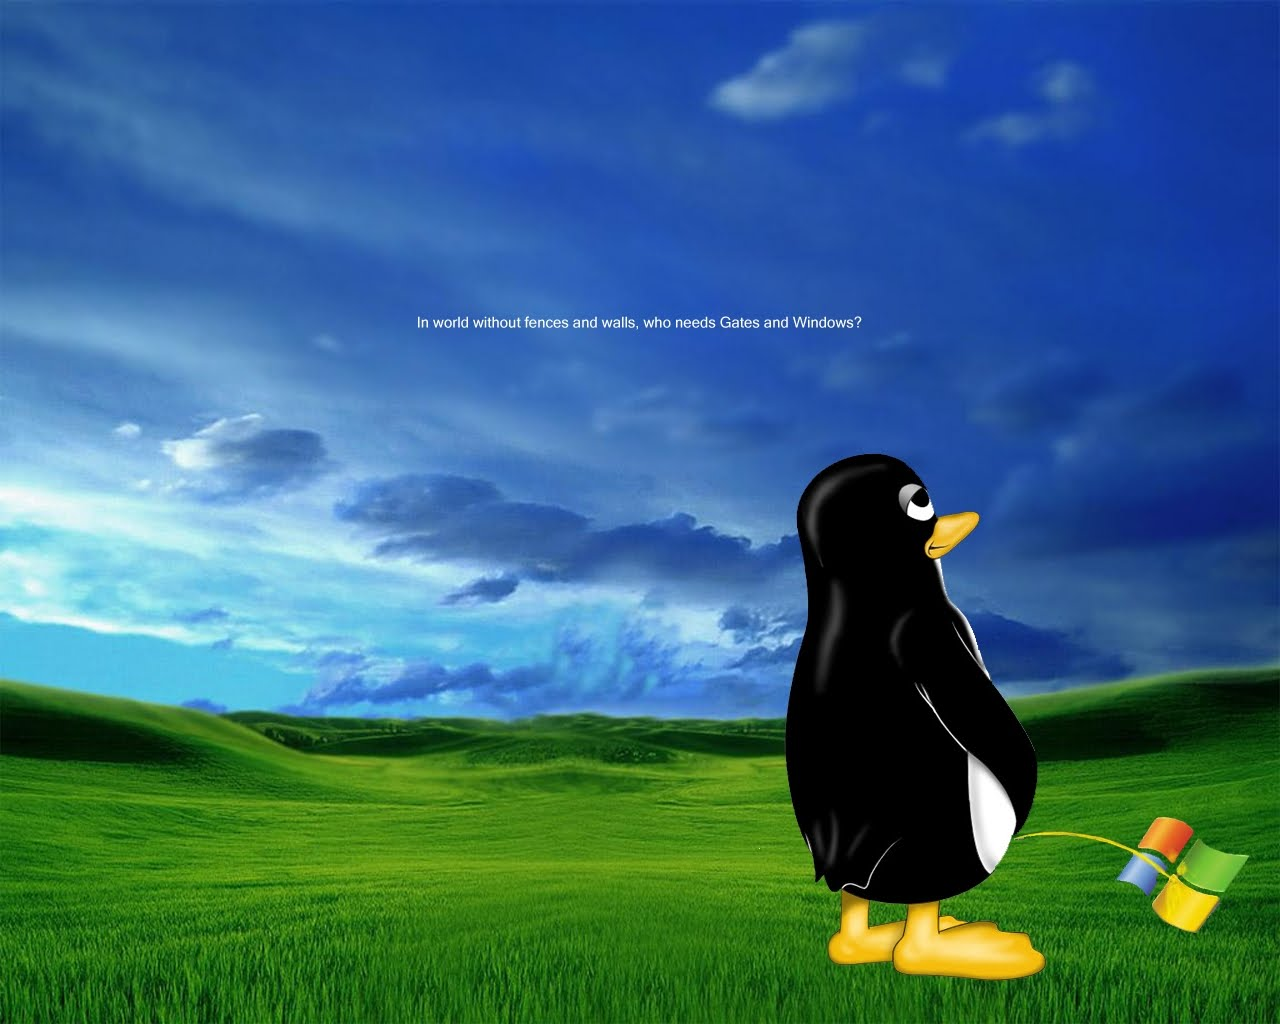
\includegraphics[width=0.7\linewidth]{tux_pee_windows}
	\end{figure}
\end{frame}

\begin{frame}
	\frametitle{Linux}
	\begin{figure}
		\centering
		
\includegraphics[width=0.7\linewidth]{linux}
	\end{figure}
\end{frame}

\subsection{Python}
\begin{frame}
	\frametitle{Python}
	\begin{figure}
		\centering
		
\includegraphics[width=0.3\linewidth]{../Resumen/python}
	\end{figure}
	\begin{figure}
		\centering
		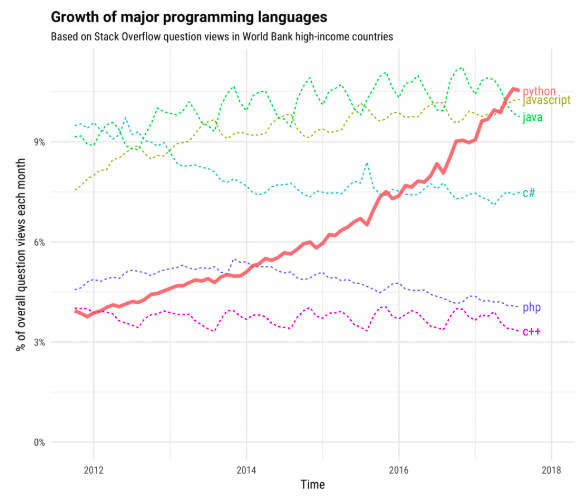
\includegraphics[width=0.7\linewidth]{../Resumen/pythontrend}
	\end{figure}
\end{frame}

\begin{frame}
	\centering
	{\LARGE Y muchos más...}
\end{frame}

\begin{frame}
	\centering
	{\LARGE Muchas Gracias por su atención}
\end{frame}

\end{document}
	